\documentclass[sigconf, anonymous, screen, pdfa]{acmart}
%==============================================================================================
% General packages before hyperref (no personalized macros here)
%=============================================================================================
\usepackage{amsmath}
	% \usepackage{amsfonts}
	% \usepackage{amssymb} % throws errors with ACM template
	% \usepackage{amsopn} % allows to define new operators, e.g., \argmin
\usepackage{mathtools}
\usepackage{graphicx} % can better scale and rotate graphics than graphic package
\usepackage{url}
\usepackage{enumitem} % remove spaces inside 'itemize' [nolistsep]

% \usepackage{bm} % bold Greek letters
\usepackage{stmaryrd} % for symbol \llceil
	% max 16 math family slots in latex; commented out bm to allow stmaryrd to work

\usepackage{upgreek} % upright Greek letters; together with package "bm" -> upright bold letters
\usepackage{bbding} % for the \CheckmarkBold symbol

\usepackage{listings} % to get sql etc nicely formatted (source code listings)
% \usepackage{fontspec} % to change the SQL font in listings
\lstset{
  basicstyle=\linespread{0.9}\ttfamily,
  columns=fullflexible,
  keepspaces=true,
  mathescape,
  escapechar={|} % https://tex.stackexchange.com/questions/345694/change-color-of-some-items-in-lstlisting  
}



\usepackage{tabularx} % table environment that allows to span a whole line
\usepackage{booktabs} % \toprule
\usepackage{multirow}
\usepackage{hhline} % cannot be overwritten by cellcolor
\usepackage{diagbox}
\usepackage{pgfplotstable} % powerful numerical table macros

	% \usepackage[usenames,table,dvipsnames,x11names]{xcolor} % not needed as options are passed directoy to documentclass 'acmart'
	% \PassOptionsToPackage{table}{xcolor} % xcolor needs to come before tikz which calls xcolor as well. Solution: pass the options before calling tikz

% for colored cells in tables
\usepackage{xcolor,colortbl}    % !!! for some reason, overleaf needs xcolor separately, although that should already have been called by colortbl (10/2019)



\usepackage{tikz} % drawing figures
\usetikzlibrary{matrix}
\usetikzlibrary{calc}
\usetikzlibrary{math}
\usetikzlibrary{arrows.meta,positioning}
\usetikzlibrary{intersections, pgfplots.fillbetween}


\usepackage{easybmat} % \begin{BMAT} alternative syntax for math tabulars and also includes the command addpath which allows to draw a path between matrix elements.

\usepackage{adjustbox}
\def\eox{\unskip\kern 10pt{\unitlength1pt\linethickness{.4pt}$\diamondsuit${}}} % "\eox" command for end of example


\usepackage{rotating}		% for rotated text in tables, \begin{turn}{75}Accuracy\end{turn}

\sloppy % Latex sometimes creates text lines that go into the margin, just to avoid ``ugly'' large spacing. The following prevents this:

\usepackage{xspace} % for macros

% \usepackage[bottom]{footmisc}   % for footnotes





%==============================================================================================
% subfigures
% use package 'subcaption'
% Package 'subfigure' is deprecated and su­per­seded by 'sub­fig' 
% But 'subfig' is not working properly with hyperref.
% 'sub­cap­tion' pack­age is most recent
% See: https://tex.stackexchange.com/questions/13625/subcaption-vs-subfig-best-package-for-referencing-a-subfigure
%=============================================================================================
\usepackage{subcaption} % recommended new package for subfigures (package subfig deprecated)
\captionsetup[figure]{labelfont=bf} % textfont=bf, labelfont=bf, ,font+=bf
\captionsetup[subfigure]{font+=small}
\captionsetup[table]{labelfont=bf} % font+=small, textfont=bf, labelfont=b

	% \captionsetup[subfigure]{justification=centering}
	\captionsetup[figure]{aboveskip=2pt}
	\captionsetup[subfigure]{aboveskip=1pt, belowskip=1pt}		% aboveskip = distance fig and subcaption)
	\captionsetup[figure]{belowskip=-3pt} % space after figures





%==============================================================================================
% Comments and ways to hide them
% macro \note{W: bla bla}: In blue. Start your comment with a short author identifier, e.g. 'W' for Wolfgang. Can be kept in the paper even during and after submission
% macro \todo{W: bla bla}: In red. Those are important issues that need to be fixed. Once they are fixed, replace the \todo with \note
% macro \mkclean: hides the blue comments (not the red ones)
%=============================================================================================
\newcommand{\todo}[1]{{{\color{red}{[\textbf{#1}]}}}} % important comments
\newcommand{\note}[1]{{{\color{magenta}{[#1]}}}} % general comments
\newcommand{\renee}[1]{{{\color{red}{#1}}}}
\newcommand{\rjm}[1]{{{\color{red}{[\textbf{RJM}: #1]}}}}

\newcommand{\revision}[1]{{\color{blue}{#1}}}



% important comments
	% \newcommand{\todo}[1]{{\sffamily{\color{red}{[\small #1]}}}} % needs to be fixed
	% \newcommand{\note}[1]{{\sffamily{\color{blue}{[\small #1]}}}} % comment
% \newcommand{\new}[1]{{\color{violet}{#1}}}

\newcommand{\hide}[1]{} 
\newcommand{\mkclean}{
    \renewcommand{\note}{\hide}
    \renewcommand{\todo}{\hide}
    \renewcommand{\rjm}{\hide}	
}


%\mkclean % comment out this line, to hide all note comments except for those that *need* to be fixed






%==============================================================================================
% ALGORITHM2e
%=============================================================================================
\usepackage[ruled,noend,linesnumbered]{algorithm2e} % boxruled, linesnumbered,ruled

\usepackage{setspace} % for setting line spacing

\DontPrintSemicolon     % does not print ";" at end of each line
	% \LinesNotNumbered
	% \LinesNumbered
\SetNlSty{}{}{}                % style of line numbers "\Setnlsty{small}{}{:}"
\SetAlgoInsideSkip{smallskip}   % distance between caption rule and beginning of algorithm
% FOLLOWING REMOVED FOR VLDB
%\SetAlCapSkip{1.5mm}             % left margin of caption
%\setlength{\algomargin}{1.5mm}    % (1) left margin of algorithm content, but also (!) right margin of caption; also puts line numbers into margin
	% \SetNlSkip{2mm}                % (2) therefore put line numbers back and use "\Indp" twice inside algorithm to put algorithm further to the right
	% \SetAlgoVlined
%\SetInd{1.5mm}{1.5mm}             % corrects for the twice usage of "\Indp"; otherwise vlines are wrong

\SetAlFnt{\small}			% size of actual algorithm text\scriptsize\sf\rm
\SetAlCapFnt{\small}		% size of name of algorithm
\SetAlCapNameFnt{\small}
% ---- For tables ----
\usepackage{array}
\usepackage{makecell}
\usepackage[utf8]{inputenc}
\def\ojoin{\setbox0=\hbox{$\bowtie$}%
  \rule[-.02ex]{.25em}{.4pt}\llap{\rule[\ht0]{.25em}{.4pt}}}
\def\leftouterjoin{\mathbin{\ojoin\mkern-5.8mu\bowtie}}
\def\rightouterjoin{\mathbin{\bowtie\mkern-5.8mu\ojoin}}
\def\fullouterjoin{\mathbin{\ojoin\mkern-5.8mu\bowtie\mkern-5.8mu\ojoin}}

% ---- OPERATORS (requires amsmath) ----



% ---- Algorithm comments ----
%\newcommand{\cc}{olive}
%\newcommand{\algocomment}[1]{\textcolor{\cc}{{//#1}}}
%\providecommand{\cc}{olive}
%\providecommand{\algocomment}[1]{\textcolor{\cc}{{//#1}}}
% ---- Notation ----


% ---- Symbols ----





%==============================================================================================
% CLEVERREF
% better than hyperref's autoref, needs to come after hyperref and algorithm2e (if referencing lines)(Sept 2015)
% \usepackage[nameinlink]{cleveref} 		% option clash with new ACM class (7/2017)
%=============================================================================================
% \usepackage[capitalise,nameinlink]{cleveref} %nameinlink makes whole word colored

% \crefname{algocf}{alg.}{algs.}
% \Crefname{algocf}{Algorithm}{Algorithms}
% \crefalias{AlgoLine}{line}%
% \crefname{proposition}{prop.}{prop.}
% \crefname{figure}{Figure}{Figures}
% \crefname{observation}{Observation}{Observations}

	% \crefformat{equation}{Eq.~(#2#1#3)}						% show reference to equation as (1)
	% \crefrangeformat{equation}{(#3#1#4) to~(#5#2#6)}
	% \crefmultiformat{equation}{(#2#1#3)}%
	% { and~(#2#1#3)}{, (#2#1#3)}{ and~(#2#1#3)}
	% 	% \crefformat{equation}{(#2#1#3)}						% show reference to equation as (1)
	% 	% \crefrangeformat{equation}{(#3#1#4) to~(#5#2#6)}
	% 	% \crefmultiformat{equation}{(#2#1#3)}%
	% 	% { and~(#2#1#3)}{, (#2#1#3)}{ and~(#2#1#3)}
	%
	% % \Crefname{equation}{Equation}{Equations}
	% \Crefformat{equation}{Equation~(#2#1#3)}						% show reference to equation as (1)




	% %==============================================================================
	% % !!! following does not work if \amsthm is used !!!
	% %
	% % These lines fix some annyong property of the ACM template that first lines of definitions
	% % swap over into the margin. Example
	% %   DEFINITION 2.4       (Actual cause).   blabla
	% % instead of
	% %   DEFINITION 2.4  (Actual cause).   blabla
	% %
	% % Solution is to tweak some distance measure in the ACM template. Below separate not to have to tweak the cls file
	% % still has to be tweaked with "~\!\!\!\!" and "~\,\," the ~ is important here (Wolf Dec 2009)
	% % remoeved for new ACM template (7/2017)
	% %==============================================================================
	% \makeatletter
	% \renewcommand{\@opargbegintheorem}[3]{%
	%    \parskip 0pt % GM July 2000 (for tighter spacing)
	%    \trivlist
	%    \item[%
	%        \hskip 10\p@
	%        \hskip \labelsep
	%        {\sc #1\ #2\             %
	%   \setbox\@tempboxa\hbox{(#3)}  %
	%        \ifdim \wd\@tempboxa>\z@ %
	%            \hskip -2\p@\relax    % This number has to be reduced from 5 !!!
	%            \box\@tempboxa       %
	%        \fi.}%
	%    ]
	%    \it
	% 	% \sloppypar	% prevents the overrun into margins of first line for theorem environments for paragraph
	% 	\setlength{\emergencystretch}{6pt}
	% }
	% \makeatother












%==============================================================================================
% New environments (notice that question and answer have slightly different formats)
% NOT NEEDED FOR acmart
% aliascnt still needed for VLDB!
%=============================================================================================
\usepackage{aliascnt}  	
	% ``hyperref’s \autoref command does not work well with theorems that share a counter:
	% it’ll always think it’s a Lemma even if it’s a Remark that shares the Lemma counter.
	% Load this package to fix it. No further intervention needed.''
	% Source: http://absatzen.de/thmtools.html (Jan 2009) 
	% better: http://www.tug.org/applications/hyperref/manual.html (Nov 2009)
	% needs also: thm-patch.sty, parseargs.sty, aliasctr.sty ???
	% see section below the three steps for usage
	% 1 define a new alias counter
	% 2 define the environment (e.g., example)      	
    % 3 reset the counter


% \newtheorem{theorem}{Theorem} % ...[section]

% \newaliascnt{corollary}{theorem}
% \newtheorem{corollary}[corollary]{Corollary}
% \aliascntresetthe{corollary}

% \newaliascnt{example}{theorem}
% \newtheorem{example}[example]{Example}
% \aliascntresetthe{example}

% \newaliascnt{definition}{theorem}
% \newtheorem{definition}[definition]{Definition}
% \aliascntresetthe{definition}

% \newaliascnt{proposition}{theorem}
% \newtheorem{proposition}[proposition]{Proposition}
% \aliascntresetthe{proposition}

% \newaliascnt{lemma}{theorem}
% \newtheorem{lemma}[lemma]{Lemma}
% \aliascntresetthe{lemma}
	
	
% \newaliascnt{conjecture}{theorem}
% \newtheorem{conjecture}[conjecture]{Conjecture}
% \aliascntresetthe{conjecture}

	% \newaliascnt{remark}{theorem}
	% \newtheorem{remark}[remark]{Remark}
	% \aliascntresetthe{remark}
	%
	% \newaliascnt{axiom}{theorem}
	% \newtheorem{axiom}[axiom]{Axiom}
	% \aliascntresetthe{axiom}
	%
	% \newaliascnt{fact}{theorem}
	% \newtheorem{fact}[fact]{Fact}
	% \aliascntresetthe{fact}
	%
	% \newaliascnt{claim}{theorem}
	% \newtheorem{claim}[claim]{Claim}
	% \aliascntresetthe{claim}




%\newtheorem{algo}[theorem]{Algorithm}

\newtheorem{observation}{Observation}
\newtheorem{problem}{Problem}
\newtheorem{answer}{Answer}
\newtheorem{question}{Question}


% ---- For tables ----
\usepackage{array}
\usepackage{makecell}
\usepackage[utf8]{inputenc}
\def\ojoin{\setbox0=\hbox{$\bowtie$}%
  \rule[-.02ex]{.25em}{.4pt}\llap{\rule[\ht0]{.25em}{.4pt}}}
\def\leftouterjoin{\mathbin{\ojoin\mkern-5.8mu\bowtie}}
\def\rightouterjoin{\mathbin{\bowtie\mkern-5.8mu\ojoin}}
\def\fullouterjoin{\mathbin{\ojoin\mkern-5.8mu\bowtie\mkern-5.8mu\ojoin}}

% ---- OPERATORS (requires amsmath) ----



% ---- Algorithm comments ----
\newcommand{\cc}{olive}
\newcommand{\algocomment}[1]{\textcolor{\cc}{{//#1}}}

% ---- Notation ----


% ---- Symbols ----















%==============================================================================================
% Make footnotesizes smaller for VLDB template
%=============================================================================================
% \let\footnotesize\scriptsize
	% \makeatletter
	% \renewcommand\footnotesize{%
	%    \@setfontsize\footnotesize\@ixpt{11}%
	%    \abovedisplayskip 8\p@ \@plus2\p@ \@minus4\p@
	%    \abovedisplayshortskip \z@ \@plus\p@
	%    \belowdisplayshortskip 4\p@ \@plus2\p@ \@minus2\p@
	%    \def\@listi{\leftmargin\leftmargini
	%                \topsep 4\p@ \@plus2\p@ \@minus2\p@
	%                \parsep 2\p@ \@plus\p@ \@minus\p@
	%                \itemsep \parsep}%
	%    \belowdisplayskip \abovedisplayskip
	% }
	% \makeatother









%==============================================================================================
% Change the color use if 'screen=true' (used in acmart.cls around line 482 (4/2019)
%==============================================================================================

\AtEndPreamble{%
    \hypersetup{colorlinks,
      linkcolor=purple,
      citecolor=blue,
      urlcolor=ACMDarkBlue,
      filecolor=ACMDarkBlue}}



%==============================================================================
% These lines fix some annyong property of the old ACM template (= VLDB template) that first lines of definitions
% swap over into the margin. Example
%   DEFINITION 2.4       (Actual cause).   blabla
% instead of 
%   DEFINITION 2.4  (Actual cause).   blabla
% Solution is to tweak some distance measure in the ACM template. Below separate not to have to tweak the cls file
% still has to be tweaked with "~\!\!\!\!" and "~\,\," the ~ is important here (Wolf Dec 2009)
%
% New fix to remove the indentation for theorems environments (Wolf July 2014)
%==============================================================================
%	\makeatletter 
%
%	\renewcommand{\@opargbegintheorem}[3]{%
%	    \parskip 0pt % GM July 2000 (for tighter spacing): 0 pt, 5 pt
%	    \trivlist
%	    \item[%
%	    	\hskip 10\p@										% this number was change to 0, former 10
%	        \hskip \labelsep
%	        {\sc #1\ #2\             % 
%	   \setbox\@tempboxa\hbox{(#3)}  % 
%	        \ifdim \wd\@tempboxa>\z@ % 
%	            \hskip 0\p@\relax    % This number has to be reduced from 5 !!!
%	            \box\@tempboxa       % 
%	        \fi.}%
%	    ]
%	    \it
%	}
%
%	\def\@begintheorem#1#2{%
%	    \parskip 0pt % GM July 2000 (for tighter spacing)
%	    \trivlist
%	    \item[%
%	    	\hskip 10\p@										% this number was change to 0, former 10
%	        \hskip \labelsep
%	        {{\sc #1}\hskip 5\p@\relax#2.}%
%	    ]
%	    \it
%	}
%
%	\makeatother






%=============================================================================================
% Nice backgroundcolor around environments and results
%=============================================================================================
\usepackage{tcolorbox}		% also allows to have shaded backgrounds around environments
\tcbuselibrary{breakable,skins}		% allow to break boxes, allow to use "enhanced jigsaw"


% === Style used for blue example environment
\tcbset{examplestyle/.style={
		enhanced jigsaw,	% if box is broken, don't show border at continuation
		colback=blue!08,	% !20	gray!10
		colframe=blue!08,	% !40
		arc=2mm,
		boxrule=0pt,		% 0pt
		% colframe=red!75!black,
		left=1mm,
		right=1mm,
		left skip= 0mm,  % breaks ACM template unless specified for specific style (4/2019)
		right skip= 0mm, % breaks ACM template unless specified for specific style (4/2019)
		top=1mm,		% 0mm, -1mm
		bottom=1mm,		% problem in package with eq at end of env. just add: \tcbset{bottom=2mm} \tcbset{bottom=0mm}
		breakable,		% allows page break
		parbox = false,		% restores normal text behavior. ELSE: paragraphs are formatted slightly different as the main text. DOWNSIDE: unwanted side effects
		% nobeforeafter,
		% before={\par\pagebreak[0]\smallskip\parindent=0pt},
		before={\par\pagebreak[0]\vspace{1mm}\parindent=0pt},		
		% before={\vspace{1mm}},			
		after={\par\pagebreak[0]\vspace{1mm}\parindent=0pt},				
		% after=5mm,		
		bottomrule = 0mm,
		boxsep = 0mm,					% common padding of hlengthi between the text content and the frame of the box, added to left, right, top, ...
		topsep at break=0pt,			% Additional vertical space at the top of middle and last parts in a break sequence
		bottomsep at break=0pt,			% Additional vertical space at the first and middle parts in a break sequence		
		pad at break=0mm,
		pad before break=1mm,		
		pad after break=1mm,		
		bottomrule at break=0mm,
		toprule at break=0mm,		
		}}

		

\usepackage{footnote}

\tcolorboxenvironment{example}{examplestyle}
%\usepackage{footnote}% allows to wrap an example in "\begin{savenotes}" to force footnotes to the bottom of page


	% \tcbset{
	% 		enhanced jigsaw,	% if box is broken, don't show border at continuation
	% 		% colback=gray!20,
	% 		% colframe=gray!40,
	% 		arc=0mm,
	% 		boxrule=1pt,		% 0pt
	% 		% colframe=red!75!black,
	% 		left=1pt,
	% 		right=1pt,
	% 		% left skip=-1pt,  % breaks ACM template (7/2018)
	% 		% right skip=-1pt, % breaks ACM template (7/2018)
	% 		topsep at break=1mm,			% Additional vertical space at the top of middle and last parts in a break sequence
	% 		top=1pt,		% 0mm, -1mm
	% 		bottom=0mm,		% problem in package with eq at end of env. just add: \tcbset{bottom=2mm} \tcbset{bottom=0mm}
	% 		breakable,		% allows page break
	% 		parbox = false		% restores normal text behavior. ELSE: paragraphs are formatted slightly different as the main text. DOWNSIDE: unwanted side effects
	% 		}

	% \tcolorboxenvironment{example}{}



% === Style used for red result box
\newcommand{\resultbox}[1]{
\begin{tcolorbox}[
	enhanced jigsaw,		% if box is broken, don't show border at continuation
	colback=red!5,
	colframe=red!75!black,	
	arc=0mm,
		% boxrule=1pt,
		% boxrule=0pt,
		% colframe=red!75!black,
	left skip=-1mm,
	right skip=-1mm,	
	left=0mm,
	topsep at break=1mm,			% Additional vertical space at the top of middle and last parts in a break sequence
		% enlarge top by=0mm,				% before box
		% enlarge top at break by=5mm,	% above box, after pagebreak
	right=0mm,
	top=0mm,
	bottom=0mm,		% problem in package with eq at end of env. justadd:\tcbset{bottom=2mm}\tcbset{bottom=0mm}
		% after skip=2mm,
	breakable,		% allows page break
		% before upper={\parindent15pt}
	parbox = false		% restores normal text behavior. ELSE: paragraphs are formatted slightly different as the main text. DOWNSIDE: unwanted side effects
]
\emph{#1}
\end{tcolorbox}
}





%==============================================================================
% defines upright \ell character as \uell (10/2014)
% Source: http://tex.stackexchange.com/questions/175236/typeset-an-upright-ell
%==============================================================================
\makeatletter
\DeclareRobustCommand*\uell{\mathpalette\@uell\relax}
\newcommand*\@uell[2]{
  % We need to adjust the width of \uell to be the same as \ell
  \setbox0=\hbox{$#1\ell$}
  \setbox1=\hbox{\rotatebox{10}{$#1\ell$}}
  \dimen0=\wd0 \advance\dimen0 by -\wd1 \divide\dimen0 by 2
  \mathord{\lower 0.1ex \hbox{\kern\dimen0\unhbox1\kern\dimen0}}
}
\makeatother






%==============================================================================
% allow figures and table to cover 100% of page
% See more: https://aty.sdsu.edu/bibliog/latex/floats.html
%==============================================================================
\renewcommand\dbltopfraction{1} %  max fraction of a two-column page that may be occupied by a (double-wide) float at top
\setcounter{dbltopnumber}{5}%  max nubmers of floats at top of two-column page (dbl = double)









%=============================================================================================
% Rebuttal
% Create marging comments for rebuttal 
% needs \usepackage{soul} for highlighting (12/2018)
%    CHANGE: now replaced soul with ulem
% "\marginpar" does not work for vldb.cls template; requires redefining it with marginnote package "\marginnote" (5/2019)
%=============================================================================================
	% \usepackage{soul} % allows strike-through and highlighting, but very fragile

    % \usepackage[normalem]{ulem} % use normalem to protect \emph; \hl command is more robust
    % \newcommand\hl{\bgroup\markoverwith
    %   {\textcolor{yellow}{\rule[-.5ex]{2pt}{2.5ex}}}\ULon}

% \newcommand{\rebuttal}[2]{\marginpar{\textbf{\textcolor{black}{#1}}}\hl{#2}}
	% \usepackage{marginnote}
	% \newcommand{\rebuttalx}[2]{\marginnote{\textbf{#1}}\hl{#2}}
	% \newcommand{\rebuttalx}[2]{\marginpar{\textbf{#2}}\hl{#1}}	# for some reason does not work: puts text in margin into yellow
	% \newcommand{\rebuttalx}[2]{\marginpar{\textcolor{black}{\textbf{#2}}}\hl{#1}}	# does not work either: puts the comment one line above
%% FOR VLDB.CLS (5/2019) 
\marginparwidth 25pt             	% Margin pars set to 0pt by vldb template
\usepackage{marginnote}
\newcommand{\rebuttal}[2]{\marginnote{\textbf{\textcolor{blue}{#1}}}{\color{blue}#2}}
    % \newcommand{\rebuttal}[2]{\marginnote{\textbf{\textcolor{black}{#1}}}\hl{#2}}

\newcommand{\reviewercomment}[1]{
\begin{tcolorbox}[
	enhanced jigsaw,		% if box is broken, don't show border at continuation
	colback=white!5,
	% colback=blue!20,
	colframe=white!75!black,	
	% colframe=gray!40,
	arc=0mm,
	% boxrule=1pt,
	% boxrule=0pt,
	% colframe=red!75!black,
	left skip=-1mm,
	right skip=1mm,	
	left=0mm,
	topsep at break=1mm,			% Additional vertical space at the top of middle and last parts in a break sequence
		% enlarge top by=0mm,				% before box
		% enlarge top at break by=5mm,	% above box, after pagebreak
	right=0mm,
	top=0mm,
	bottom=0mm,		% problem in package with eq at end of env. justadd:\tcbset{bottom=2mm}\tcbset{bottom=0mm}
		% after skip=2mm,
	breakable,		% allows page break
		% before upper={\parindent15pt}
	parbox = false		% restores normal text behavior. ELSE: paragraphs are formatted slightly different as the main text. DOWNSIDE: unwanted side effects
]
\emph{#1}
\end{tcolorbox}
}

\newcommand{\high}[1]{\textup{\textbf{#1.}}}







%==============================================================================================
% Other macros (add here your personalized macros)
%=============================================================================================
\newcommand{\smallsection}[1]{\vspace{2mm}\noindent\textbf{#1.}} % new subsection type: noindent, bold
\newcommand{\introparagraph}[1]{\textbf{#1.}} % define own new subsection type: noindent, bold (textsc)

\newcommand{\ourmethod}{\textsc{OurMethod}\xspace}
\renewcommand{\epsilon}{\varepsilon} % nicer epsilon symbol
\newcommand{\set}[1]{\{#1\}}                    % Set (as in \set{1,2,3}).
\newcommand{\setof}[2]{\{{#1}\mid{#2}\}}        % Set (as in \setof{x}{x>0}).

\newcommand{\define}{:=} % define symbol
	% \newcommand{\define}{\stackrel{\textup{\tiny def}}{=}}
	% \newcommand{\define}{\triangleq} % define symbol

\newcommand{\datarule}{{\,:\!\!-\,}} % datalog command (March 2010)
\renewcommand{\vec}[1]{\boldsymbol{\mathbf{#1}}}
%\newcommand{\transpose}{\intercal}	% alternatives: \top \intercal

\newcommand{\N}{\mathbb{N}} % Natural numbers
\newcommand{\R}{{\mathbb{R}}} % Real numbers
\newcommand{\bigO}{{\mathcal{O}}} % Big O notation
\newcommand{\bigTH}{{\mathcal{\Theta}}} % Big O notation
\renewcommand{\O}{{\mathcal{O}}} % Big O notation DEPRECATED
\renewcommand{\P}{{\mathbb{P}}} % Probability \P
\newcommand{\PP}[1]{\mathbb{P} [ #1 ]} % Probability \PP{} -> P[], hollow
\newcommand{\E}{\mathbb{E}}
\newcommand{\sql}[1]{\textup{\textsf{\small#1}}}
\newcommand{\datastyle}[1]{\texttt{#1}}


% \newcommand{\val}{\textup{\textrm{cost}}}
\newcommand{\val}{\textup{\textrm{val}}}
% \newcommand{\val}{w}
\newcommand{\var}[1]{{\textup{\texttt{var}}} ( #1 )}  % May 2011 (note naming conflict with variables !!!)
\newcommand{\Var}{\textup{\texttt{Var}}}		






%%%%%%%%%%%%%%%%%%%%%%%%%%%%%%%%%%%%%%%%%%%%%%%%%%%%%%%%%%%%%%%%%%%%%%%%%%%%%%%%
%%%% ORCID icons for authors. Needs to have the image file too in dunnemacros/
%%%%%%%%%%%%%%%%%%%%%%%%%%%%%%%%%%%%%%%%%%%%%%%%%%%%%%%%%%%%%%%%%%%%%%%%%%%%%%%%

% % Use to create orcid icons and links for authors
% % Usage: \orcidicon{<NAME>}{<ORCID>}
% \newcommand{\orcidicon}[2]{%
%   %\hypersetup{urlcolor=black}}{}% don't add colored links to author names
% %  \begingroup\normalfont
%   \href{#2}{#1 \includegraphics[height=\fontcharht\font`\B]{figs/orcid_16x16.png}}%
% }

\usepackage{scalerel}
\usepackage{tikz}
\usetikzlibrary{svg.path}

\definecolor{orcidlogocol}{HTML}{A6CE39}
\tikzset{
  orcidlogo/.pic={
    \fill[orcidlogocol] svg{M256,128c0,70.7-57.3,128-128,128C57.3,256,0,198.7,0,128C0,57.3,57.3,0,128,0C198.7,0,256,57.3,256,128z};
    \fill[white] svg{M86.3,186.2H70.9V79.1h15.4v48.4V186.2z}
                 svg{M108.9,79.1h41.6c39.6,0,57,28.3,57,53.6c0,27.5-21.5,53.6-56.8,53.6h-41.8V79.1z M124.3,172.4h24.5c34.9,0,42.9-26.5,42.9-39.7c0-21.5-13.7-39.7-43.7-39.7h-23.7V172.4z}
                 svg{M88.7,56.8c0,5.5-4.5,10.1-10.1,10.1c-5.6,0-10.1-4.6-10.1-10.1c0-5.6,4.5-10.1,10.1-10.1C84.2,46.7,88.7,51.3,88.7,56.8z};
  }
}

\RequirePackage{etoolbox}
\DeclareRobustCommand\orcidicon[1]{\href{https://orcid.org/#1}{\mbox{\scalerel*{

\begin{tikzpicture}[yscale=-1,transform shape]
\pic{orcidlogo};
\end{tikzpicture}
}{|}}}}

%rjm outerjoins
\def\ojoin{\setbox0=\hbox{$\bowtie$}%
  \rule[-.02ex]{.25em}{.4pt}\llap{\rule[\ht0]{.25em}{.4pt}}}
\def\leftouterjoin{\mathbin{\ojoin\mkern-5.8mu\bowtie}}
\def\rightouterjoin{\mathbin{\bowtie\mkern-5.8mu\ojoin}}
\def\fullouterjoin{\mathbin{\ojoin\mkern-5.8mu\bowtie\mkern-5.8mu\ojoin}}

%rjm nulls
%\def\missing{\mathbin{\perp \perp}}
%\def\missing{\mathbin{\hat{\perp}}}
\def\missing{\mathbin{\pm}}
\def\produced{\mathbin{\perp}}
\def\schema{\mathbin{\mathcal{A}}}
%\def\schema{\mathbin{sc}}



% ---- For tables ----
\usepackage{array}
\usepackage{makecell}
\usepackage[utf8]{inputenc}
\def\ojoin{\setbox0=\hbox{$\bowtie$}%
  \rule[-.02ex]{.25em}{.4pt}\llap{\rule[\ht0]{.25em}{.4pt}}}
\def\leftouterjoin{\mathbin{\ojoin\mkern-5.8mu\bowtie}}
\def\rightouterjoin{\mathbin{\bowtie\mkern-5.8mu\ojoin}}
\def\fullouterjoin{\mathbin{\ojoin\mkern-5.8mu\bowtie\mkern-5.8mu\ojoin}}

% ---- OPERATORS (requires amsmath) ----



% ---- Algorithm comments ----


% ---- Notation ----

%rjm feel free to change the definition of this macro
%\newcommand{\arx}{Archive}
\newcommand{\arx}{arXiv}
\newcommand{\so}{S2ORC}
%\newcommand{\so}{Semantic Scholar}


\newcommand{\ours}{$MLB$}
\newcommand{\transpose}{$MLB_T$}
\newcommand{\header}{$MLB_H$}

% ---- Symbols ----

   % lab template macros (Data_Intelligence_Template)
%==============================================================================================
% KeyRing paper-specific macros.
% Load after datalabmacros.tex (the lab template). Add only what the lab macros do not provide.
%=============================================================================================

% ---- System name: change it only here; the text uses \ourmethod (lab convention) ----
\renewcommand{\ourmethod}{\textsc{KeyRing}\xspace}
\newcommand{\sys}{\ourmethod} % alias; the figures, which do not load the lab macros, define \sys themselves

% ---- Packages used by this paper and not loaded by datalabmacros ----
\usepackage{balance} % \balance before the bibliography

% ---- Table 1 helpers (bbding is loaded by datalabmacros) ----
\newcommand{\cmark}{\CheckmarkBold}
\newcommand{\xmark}{\XSolidBrush}
\newcolumntype{Y}{>{\raggedright\arraybackslash}X}
\definecolor{sysbg}{gray}{0.92}

% ---- Layout ----
\def\shorten{\looseness=-1} % pull a paragraph up by one line when possible

% ---- Aliases for older drafts (map to lab macros) ----
\newcommand{\blue}[1]{\revision{#1}}
\newcommand{\eat}[1]{\hide{#1}}
  % paper-specific macros


% Submission front matter for SIGMOD'28 (anonymous review)
\settopmatter{printacmref=true, printfolios=true}
\setcopyright{rightsretained}
\makeatletter\@printpermissionfalse\makeatother
\copyrightyear{2028}
\acmYear{2028}
\acmISBN{978-1-4503-XXXX-X/2018/06}
\acmDOI{XXXXXXX.XXXXXXX}
\acmConference[SIGMOD'28]{SIGMOD}{2028}{TBD} % TODO: SIGMOD'28 dates and location

\begin{document}

\title[KeyRing: Scalable Join Discovery with LLMs and Recall Guarantees]{KeyRing: Scalable Join Discovery with LLMs\\ and Recall Guarantees}
% Alternatives:
% \title{From Table Pairs to Key Domains: Cost-Efficient LLM-Assisted Join Discovery}
% \title{KeyRing: Discovering Join Keys across Thousands of Tables with Few LLM Calls}
% \title{KeyRing: Cost-Efficient LLM-Assisted Join Discovery via Key Domains}
% Previous: KeyRing: LLM-Assisted Join Key Discovery over Thousands of Tables at the Cost of Key Domains, not Table Pairs


\author{Anonymous Author(s)}
\affiliation{\institution{}\country{}}

\begin{abstract}
% 1. State the problem
Analytics, BI, and LLM agents over enterprise data first need a join graph: which tables join, on which keys, and in which direction.
Each business in an enterprise platform has 50 to 8K tables, rarely declares these keys, and keeps adding tables.
% 2. Say why it's an interesting problem
Non-LLM methods, such as inclusion-dependency discovery, learned foreign-key detectors, and joinable-table search, are cheap but decide joins from value overlap and names alone.
They accept accidental overlaps of surrogate IDs, codes, and dates, and they miss true joins whose values are only partially contained or formatted differently.
LLM-based methods add the semantics these methods lack, but current practice sends every pair of tables to the LLM: about 32M calls for 8K tables, and almost all of them return ``no join''.
Each new table then costs one more prompt for every existing table.
Hybrid methods cluster tables by topic or route each pair through a cheap proxy before the LLM, but topics are not key domains, proxies inherit the failures of non-LLM signals, and every pair is still judged independently.
% 3. Say what your solution achieves
We present \ourmethod, a hybrid system that discovers join keys with LLM calls proportional to the number of \emph{key domains}, not the number of table pairs.
\ourmethod builds on the observation that enterprise joins concentrate on a few key domains, such as customer or project identifiers, that many tables share.
\ourmethod uses non-LLM signals for what they do well: it profiles every column once, generates candidates with indexes, and groups candidate key columns into \emph{rings}, one per key domain.
It uses the LLM for what only the LLM does well: it verifies the semantics of each ring once, together with a few uncertain candidates.
A cost-based optimizer routes each candidate to a local model distilled from earlier LLM decisions or to the LLM, so that \ourmethod keeps a target recall of the all-pairs LLM baseline with a user-given confidence.
Joins follow from ring membership, so the resulting graph is a star around each key owner instead of a clique of redundant edges.
\ourmethod runs online: when a table arrives, it looks up the new columns in its indexes and verifies only the rings they affect, so the cost of an arrival does not grow with the number of tables.
% 4. Say what follows from your solution
On \todo{N} enterprise databases with up to \todo{8K} tables and on public benchmarks, \ourmethod improves join F1 over the best non-LLM method by \todo{P} points, and reduces LLM calls by \todo{X}$\times$ and tokens by \todo{Y}$\times$ compared to all-pairs prompting, while keeping \todo{Z}\% of its joins.
When tables arrive one at a time, \ourmethod adds each table with \todo{V}$\times$ fewer LLM calls than pairwise prompting and returns the same graph as a batch run.
\end{abstract}

%%
%% The code below is generated by the tool at http://dl.acm.org/ccs.cfm.
%% Please copy and paste the code instead of the example below.
%%
% \begin{CCSXML}
%     <ccs2012>
%      <concept>
%       <concept_id>00000000.0000000.0000000</concept_id>
%       <concept_desc>Do Not Use This Code, Generate the Correct Terms for Your Paper</concept_desc>
%       <concept_significance>500</concept_significance>
%      </concept>
%      <concept>
%       <concept_id>00000000.00000000.00000000</concept_id>
%       <concept_desc>Do Not Use This Code, Generate the Correct Terms for Your Paper</concept_desc>
%       <concept_significance>300</concept_significance>
%      </concept>
%      <concept>
%       <concept_id>00000000.00000000.00000000</concept_id>
%       <concept_desc>Do Not Use This Code, Generate the Correct Terms for Your Paper</concept_desc>
%       <concept_significance>100</concept_significance>
%      </concept>
%      <concept>
%       <concept_id>00000000.00000000.00000000</concept_id>
%       <concept_desc>Do Not Use This Code, Generate the Correct Terms for Your Paper</concept_desc>
%       <concept_significance>100</concept_significance>
%      </concept>
%     </ccs2012>
%     \end{CCSXML}
    
%\keywords{Automatic Data Processing; Pipeline Generation}
%\ccsdesc[500]{Information systems~Database management system engines}
%\ccsdesc[500]{Information systems~Data processing}
%\ccsdesc[500]{Information systems~Automatic data processing}
%\ccsdesc[500]{Theory of computation~Database query processing and optimization (theory)}


%\received{July 2024}
%\received[revised]{Septemer 2024}
%\received[accepted]{October 2024}

\maketitle

\section{Introduction}
\label{sec:introduction}

Enterprise data platforms ingest the databases of many business units, ERP systems, and exported files.
Before analysts, BI tools, or LLM agents can query this data, the platform needs a \emph{join graph}: which tables join, on which key columns, and in which direction.
Text-to-SQL over large schemas~\cite{Spider2} and automatic BI modeling~\cite{AutoBI} both depend on it.
However, enterprise databases rarely declare foreign keys.
Tables arrive as staging copies, snapshots, and exports, and one business can have 50 to 10K tables.
The join graph must therefore be discovered from the data and its metadata.

\introparagraph{Example} Consider a project-based services firm with \todo{2,010} tables.
A \emph{project code} identifies a project in the project master table, and \todo{k} other tables reference it: ledgers, timesheets, invoices, budgets, and their staging copies and snapshots.
In some tables the column is called \texttt{PROJECT\_CODE}, in others \texttt{PRJ\_ID} or \texttt{ENGAGEMENT}.
Staging copies keep only recent projects, and one export pads codes with leading zeros.
At the same time, dozens of tables have auto-increment surrogate columns that start at 1, status columns with values 1 to 5, and a generic column named \texttt{DATA}.
A correct join graph links the \todo{k} referencing columns to the project master, and nothing else.

\introparagraph{Non-LLM Join Discovery} The classic approach decides joins from data statistics.
Inclusion-dependency algorithms find columns whose values are contained in a unique column~\cite{Tschirschnitz17}.
Learned detectors score such candidates with features such as uniqueness, containment, and name similarity~\cite{Rostin09,ZhangHOPS10,HoPF}, and Auto-BI~\cite{AutoBI} combines a local join classifier with a global graph optimization.
Joinable-table search treats each column as a \emph{domain}, the set of its distinct values, and finds the columns whose domains overlap most with a query column.
LSH Ensemble~\cite{DBLP:journals/pvldb/ZhuNPM16} showed that set containment $|Q \cap X|/|Q|$, not Jaccard similarity, is the right overlap measure when domain sizes are skewed, and indexes it with MinHash sketches at the scale of hundreds of millions of domains.
JOSIE~\cite{DBLP:conf/sigmod/ZhuDNM19}, MATE~\cite{MATE}, DeepJoin~\cite{2023_dong_deepjoin}, and Freyja~\cite{Freyja} extend this search to exact overlap, multi-column keys, embeddings, and learned join quality.
These methods are cheap and scale to large data lakes.
However, on the example above they fail in four ways.
\begin{itemize}[leftmargin=*]
\item \textbf{Accidental overlap creates false joins.} Every surrogate column with values $1..m$ is contained in every other surrogate column with values $1..n$, $n \geq m$. Status codes, years, and flags overlap in the same way. Value statistics cannot distinguish these overlaps from real references, so the graph fills with false edges. LakeBench~\cite{LakeBench} reports the same failure for joinable-table search: JOSIE returns a column of street names for a query column of last names, because both contain values such as ``Lincoln'' and ``Washington''. In our databases, \todo{P}\% of the inclusion dependencies with containment above 0.9 are not joins.
\item \textbf{Real joins look imperfect.} Staging copies, deleted rows, and snapshots make containment partial, and formatting differences, such as leading zeros or prefixes, make it zero. A strict containment threshold misses these joins, and a loose one admits more accidental overlaps. No single threshold works across a database.
\item \textbf{Names do not carry meaning.} The same key appears under different names (\texttt{PRJ\_ID}, \texttt{ENGAGEMENT}), and different keys share generic names (\texttt{ID}, \texttt{CODE}, \texttt{DATA}). String similarity on names cannot resolve either case. The column descriptions and business context that would resolve them are text that these methods do not read.
\item \textbf{Learned models do not transfer.} Learned detectors and Auto-BI need labeled joins from schemas similar to the target. Every business has its own naming conventions and source systems, and labels are expensive: LakeBench~\cite{LakeBench} spent more than 7,500 human hours to label its join and union queries. Joinable-table search returns a ranked list per query column, not a decision with a key direction.
\end{itemize}

\introparagraph{LLM-based Join Discovery} LLMs address these failures because they read column names, descriptions, and sample values together, and they bring knowledge of common business entities~\cite{dataWrangleNarayan2022}.
An LLM can tell that \texttt{ENGAGEMENT} holds project codes and that a surrogate \texttt{ID} does not reference a status table.
Current practice therefore sends every pair of tables (source and target) to an LLM, which decides whether the pair joins and returns the key.
This approach is accurate, but its cost grows quadratically with the number of tables.
A business with $n$ tables needs $n(n-1)/2$ LLM calls: about 500K calls for 1K tables and about 50M calls for 10K tables.
Each call carries two schemas and sample rows, so a single business costs \todo{\$X} in tokens and \todo{Y} hours of inference.
The calls are also mostly wasted: only \todo{Z}\% of the table pairs in our databases join.
In the example, the LLM is asked about each of the $\binom{k+1}{2}$ pairs among the project tables, although the answers follow from the $k$ references to the project master.
Independent answers can also contradict each other, and they add a clique of redundant edges to the join graph.

\introparagraph{Hybrid Join Discovery} A natural fix is to combine cheap methods with the LLM.
Hybrids do so in two ways.

The first way \emph{narrows the search space} before the LLM.
Schuyler~\cite{Schuyler} clusters the tables of a database into topics with self-supervised LLM embeddings, and notes that such clusters reduce the search for joinable tables to matching within and across groups.
Our production pipeline follows the same idea: an LLM tags each table and groups related tables into concepts before it searches for joins.
Magneto~\cite{Magneto} uses a small model to retrieve candidate column matches for an LLM.
However, topics are not key domains.
A customer or project key crosses topic boundaries, so restricting the search to a cluster loses joins, and searching across clusters brings back the quadratic number of pairs.

The second way \emph{routes each pair} to a cheap proxy or to the LLM.
Semantic join operators in LOTUS~\cite{LOTUS} and Palimpzest~\cite{Palimpzest}, and model cascades~\cite{FrugalGPT}, accept or reject a pair by its embedding similarity and defer inconclusive pairs to the LLM.
SUPG~\cite{SUPG} and BARGAIN~\cite{BARGAIN} set the deferral thresholds so that the result keeps a target precision or recall of the LLM with statistical guarantees.
Such cascades save little when embeddings do not encode the join condition: on real data, BARGAIN still defers about 80\% of pairs to the LLM~\cite{FDJ}.
Featurized-Decomposition Join (FDJ)~\cite{FDJ} reduces the cost by up to $10\times$ with a key idea: extract features from each record with a linear pass of the LLM, and decide the join with cheap comparisons on those features.

These hybrids lower the cost per pair, but they inherit two problems.
First, a cheap filter or proxy inherits the failures of non-LLM methods: a surrogate overlap passes it and costs an LLM call, and a real join with zero containment is dropped before the LLM sees it.
Second, they evaluate a given join predicate over record pairs of two given tables.
Join discovery asks a different question: which of thousands of tables join, and on which of their columns.
Applied to table or column pairs, these operators judge every pair independently.
They do not use what makes join keys special: one side is unique, the other side references it, and many tables share one key domain.
The number of LLM calls still grows with the number of candidate pairs.

\begin{table}[t]
\centering
\scriptsize
\setlength{\tabcolsep}{2.5pt}
\setlength{\aboverulesep}{0pt}
\setlength{\belowrulesep}{0pt}
\renewcommand{\arraystretch}{1.35}
\caption{Join key discovery over thousands of tables: non-LLM methods
are cheap but decide from overlap and names, all-pairs LLM prompting
calls the LLM per table pair, hybrids still judge pairs independently;
\ourmethod calls the LLM per key domain and keeps a target recall.}
\label{tab:intro-landscape}
\begin{tabularx}{\columnwidth}{@{}>{\raggedright\arraybackslash}p{1.4cm}YYYY>{\columncolor{sysbg}}Y@{}}
\toprule
 & \multicolumn{2}{c}{\textbf{Non-LLM}}
 & \textbf{LLM}
 & \textbf{Hybrid}
 & \textbf{Hybrid} \\
\cmidrule(lr){2-3}
 & \textbf{Auto-BI}~\cite{AutoBI}
 & \textbf{JOSIE}~\cite{DBLP:conf/sigmod/ZhuDNM19}
 & \textbf{All-pairs}\newline prompting
 & \textbf{LOTUS}~\cite{LOTUS},\newline \textbf{FDJ}~\cite{FDJ}
 & \textbf\ourmethod\newline ours \\
\midrule
\textbf{Robust to accidental overlap}
 & \xmark{} learned syntactic features
 & \xmark{} value overlap
 & \cmark{}
 & \cmark{} if routed to LLM
 & \cmark{} LLM checks each ring \\
\cmidrule{1-6}
\textbf{Finds joins with partial or zero containment}
 & \xmark{}
 & \xmark{}
 & \cmark{}
 & \xmark{} if proxy drops them
 & \cmark{} normalized formats, embeddings \\
\cmidrule{1-6}
\textbf{Labeled data needed}
 & \xmark{} corpus of BI models
 & \cmark{} none
 & \cmark{} none
 & \cmark{} none
 & \cmark{} own LLM decisions \\
\cmidrule{1-6}
\textbf{LLM calls grow with}
 & n/a
 & n/a
 & \xmark{} table pairs
 & \xmark{} candidate pairs
 & \cmark{} key domains \\
\cmidrule{1-6}
\textbf{Recall guarantee}
 & \xmark{}
 & \xmark{} top-$k$ by overlap
 & n/a (asks all pairs)
 & \cmark{} per operator
 & \cmark{} vs.\ all-pairs LLM \\
\cmidrule{1-6}
\textbf{Returns key and direction}
 & \cmark{}
 & \xmark{}
 & \cmark{}
 & \xmark{} user predicate
 & \cmark{} owner and members \\
\cmidrule{1-6}
\textbf{Consistent, non-redundant graph}
 & \cmark{} arborescence
 & \xmark{}
 & \xmark{} independent answers
 & \xmark{}
 & \cmark{} star per key domain \\
\cmidrule{1-6}
% TODO(Saeed): fill from the experiments on the largest production database.
\textbf{F1; cost} (\todo{N} tables)
 & \todo{F1}; no LLM
 & \todo{F1}; no LLM
 & \todo{F1}; \todo{\$, h}
 & \todo{F1}; \todo{\$, h}
 & \todo{F1}; \todo{\$, h} \\
\bottomrule
\end{tabularx}
\end{table}


\introparagraph{Problem and Challenges} Given a database without declared keys and an LLM, we aim to discover its join keys with as few LLM calls as possible, while keeping a target recall of the all-pairs LLM baseline.
Table~\ref{tab:intro-landscape} compares one representative per category against this goal.
Meeting it is hard for three reasons.
First, the candidate space is quadratic and almost all of it is empty, so pruning must remove nearly all pairs before any LLM call, yet every true join it drops is lost silently.
Second, the cheap signals that pruning relies on are exactly the ones that fail in non-LLM methods.
Third, pairwise decisions ignore the structure of key domains, so they are redundant and can be inconsistent.

\introparagraph{Our Insight} Enterprise joins are not spread evenly over table pairs.
They concentrate on a small number of \emph{key domains}, such as customer, project, employee, or invoice identifiers.
Each key domain has one \emph{owner} column that is unique, and many \emph{member} columns that reference it.
If we know the key domains, we know the joins: every member joins with its owner.
The number of key domains is orders of magnitude smaller than the number of table pairs.
So the LLM should verify key domains, not pairs.
This lifts FDJ's insight from records to schemas: work that is linear in the number of columns (profiling, annotation, and grouping columns into key domains) replaces work that is quadratic in the number of tables.
It also extends the value domains of LSH Ensemble with meaning and ownership: a key domain is a set of columns that refer to the same business entity, with one owner.
Finally, it splits the work between the two kinds of methods along their strengths.
Non-LLM signals are reliable for uniqueness and for proposing candidates with high recall, but not for deciding meaning.
The LLM is reliable for meaning, but too expensive to apply to every pair.

\introparagraph{System Overview} This paper presents \ourmethod\footnote{\ourmethod holds all columns of one key domain together, like keys on a ring. The code is available to reviewers at \url{https://anonymous.4open.science/r/KeyRing}.}, a hybrid system that discovers join keys with LLM calls proportional to the number of key domains.
\ourmethod has three components.
First, the \emph{Column Profiler} reads the data once and computes sketches of each column's values, its uniqueness, type, value pattern, and normalized formats, and an embedding of its name and description.
No later step reads raw data.
Second, the \emph{Ring Builder} generates candidates with containment and embedding indexes, tuned for recall rather than precision.
It prunes generic and type-incompatible columns, and groups the remaining columns into \emph{rings}, one per candidate key domain, each with an elected owner.
Third, the \emph{Budgeted Verifier} decides which rings and candidates need the LLM.
A local model, distilled from \ourmethod's own earlier LLM decisions rather than from labeled schemas, accepts or rejects confident candidates.
The LLM verifies each ring once, in a batched prompt with its owner, its members, and its uncertain candidates, and removes accidental members such as surrogate overlaps.
A cost-based optimizer chooses thresholds and batches so that \ourmethod keeps a target recall $\gamma$ of the all-pairs LLM baseline with probability at least $1-\delta$.
Confirmed rings propagate joins by transitivity without further LLM calls.
The output join graph is a star around each owner, not a clique of redundant edges.

\introparagraph{Contributions} Our primary contribution is \ourmethod, a holistic and practical hybrid system for join key discovery over thousands of tables that is more accurate than non-LLM methods and whose LLM cost grows with the number of key domains, not with the number of table pairs.
Our detailed technical contributions are:
\begin{itemize}[leftmargin=*]
\item An analysis of why non-LLM, LLM-based, and hybrid join discovery fail on enterprise databases, a formalization of cost-bounded join key discovery with a recall target relative to an LLM oracle, and a system architecture that solves it by discovering key domains instead of judging table pairs (Sections~\ref{sec:background} and~\ref{sec:architecture}).
\item A ring builder that turns one pass of column profiling into key-domain candidates with elected owners, using containment and embedding indexes, format normalization, and pruning of generic columns (Section~\ref{sec:ring_builder}).
\item A budgeted verifier that combines a distilled local model, batched LLM prompts per ring, and transitive propagation, and a cost-based optimizer that meets a recall target with statistical guarantees (Section~\ref{sec:verifier}).
\item A comprehensive evaluation on \todo{N} production enterprise databases with up to \todo{10K} tables and on public benchmarks, against non-LLM methods (inclusion-dependency discovery, Auto-BI, joinable-table search), all-pairs LLM prompting, and hybrid methods (Section~\ref{sec:experiments}). \ourmethod improves join F1 over the best non-LLM method by \todo{P} points, and reduces LLM calls by \todo{X}$\times$, tokens by \todo{Y}$\times$, and end-to-end time by \todo{W}$\times$ compared to all-pairs prompting, while keeping \todo{Z}\% of its joins.
\end{itemize}

\section{Background and Problem Formulation}
\label{sec:background}
In this section, we review the three categories of join discovery from Table~\ref{tab:intro-landscape}: non-LLM, LLM-based, and hybrid.
For each category, we describe how it decides joins and where it falls short on enterprise databases.
We then review how profiling metadata is collected and provided to LLMs, and formalize cost-bounded join key discovery.

\subsection{Non-LLM Join Discovery}
\label{sec:bg_nonllm}
Non-LLM methods decide joins from data statistics and schema metadata.
They fall into two groups: key and inclusion-dependency discovery, which decides joins inside one database, and joinable-table search, which ranks candidate columns for a query column in a data lake.

\introparagraph{Key and Inclusion-Dependency Discovery} A unary \emph{inclusion dependency} (IND) $A \subseteq B$ holds if every value of column $A$ also appears in column $B$.
If $B$ is also unique, then $A$ is a foreign-key candidate that references $B$.
IND discovery algorithms check this condition for all column pairs, and scale to databases with very many tables by sorting and sharing value sets across checks~\cite{Tschirschnitz17}.
Real data rarely satisfies exact INDs, so approximate INDs relax the condition to a containment threshold.
Every IND is only a candidate, and most candidates are not foreign keys.
Learned detectors therefore rank candidates with features, such as the uniqueness of $B$, the containment of $A$ in $B$, the similarity of column names, and the distribution of values~\cite{Rostin09,ZhangHOPS10}.
HoPF~\cite{HoPF} detects primary and foreign keys together, so that a column chosen as a primary key constrains which foreign keys may reference it.
Auto-BI~\cite{AutoBI} goes one step further.
It first trains a local classifier that predicts, for each column pair, whether it is an N:1 join.
It then selects a global join graph that maximizes the combined classifier scores under structural constraints, a variant of the minimum-cost arborescence problem.
The global step removes many locally plausible but inconsistent joins.

\introparagraph{Joinable-Table Search} Data lake systems treat each column as a \emph{domain}, the set of its distinct values, and rank the columns of a lake by their overlap with a query column.
LSH Ensemble~\cite{DBLP:journals/pvldb/ZhuNPM16} uses set containment $|Q \cap X| / |Q|$ as the overlap measure.
Unlike Jaccard similarity, containment does not penalize a large domain $X$ for values outside $Q$, which matters because domain sizes follow a power-law distribution.
LSH Ensemble indexes MinHash sketches of all domains in partitions of similar size, and answers containment queries over hundreds of millions of domains in seconds.
JOSIE~\cite{DBLP:conf/sigmod/ZhuDNM19} returns the exact top-$k$ columns by set overlap and chooses between reading posting lists and reading candidate sets with a cost model.
MATE~\cite{MATE} extends the search to multi-column keys.
DeepJoin~\cite{2023_dong_deepjoin} embeds columns with a pre-trained language model and searches them with an approximate nearest-neighbor index, which also finds joins with similar but not identical values.
Freyja~\cite{Freyja} learns a join quality metric from column profiles instead of raw values.

\introparagraph{Limitations} Non-LLM methods are cheap, but they decide joins from syntactic evidence, and enterprise databases defeat this evidence in four ways.
First, accidental overlap creates false joins.
Surrogate keys that count from 1, status codes, years, and flags are contained in each other, and a unique surrogate column looks like a valid target for all of them.
LakeBench~\cite{LakeBench} shows the same problem for joinable-table search: a column of street names overlaps a query column of last names, and JOSIE ranks it among the top results although the two columns are not joinable.
Second, real joins look imperfect.
Staging tables, snapshots, and deleted rows make containment partial, and formatting differences make exact overlap zero.
On LakeBench queries whose joins have only fuzzy overlap, JOSIE reaches 0\% top-10 accuracy and DeepJoin reaches 33\%~\cite{LakeBench}.
LakeBench concludes that no method is effective in all cases, because joinable columns must both mean the same thing and overlap in value~\cite{LakeBench}.
Third, names do not resolve meaning.
One key appears under different names, and different keys share generic names such as \texttt{ID}, \texttt{CODE}, or \texttt{DATA}.
Column descriptions and business context would resolve these cases, but these methods do not read them.
Fourth, learned models need labels.
The detectors and Auto-BI learn from labeled joins, and labels for a new enterprise schema are expensive: LakeBench spent more than 7,500 human hours to label its queries~\cite{LakeBench}.
Joinable-table search, in turn, returns a ranked list per query column, not a join decision with a key direction.

\subsection{LLM-based Join Discovery}
\label{sec:bg_llm}
LLMs decide what columns mean.
Foundation models match entities and schema elements across tables without task-specific training~\cite{dataWrangleNarayan2022}, and they read names, descriptions, and sample values together.
This resolves the cases that defeat non-LLM methods: an LLM recognizes that \texttt{ENGAGEMENT} holds project codes, that a surrogate \texttt{ID} does not reference a status table, and that a street name is not a last name.

\introparagraph{All-Pairs Prompting} Current practice in enterprise data platforms, including the production pipeline we study, discovers joins in three LLM steps.
First, the LLM annotates every table: it tags its columns with semantic types and writes a description.
Second, it tags each table with the \emph{concepts} of a business data model, such as project or invoice, whose data the table holds.
Third, it discovers joins pair by pair.
For each pair of tables, one prompt removes the columns that cannot be keys, a second prompt selects the candidate key columns of one table, and one further prompt per candidate lists all columns of the other table with their descriptions and sample values and returns the matching columns.
Warehouse queries then score the matches by value overlap and uniqueness and assemble a composite key greedily.
The first two steps make one LLM call per table or per batch of tables, so their cost is linear in the number of tables.
The third step dominates the cost.

\introparagraph{Limitations} All-pairs prompting is accurate, but it faces four limitations.
First, its cost grows quadratically.
A database with $n$ tables needs $n(n-1)/2$ pair evaluations, about 32M for 8K tables, and each evaluation makes $2 + c$ LLM calls for $c$ candidate columns, most of which carry a full schema and sample values.
In our databases, only \todo{Z}\% of the pairs join, so almost all calls return ``no join''.
Second, its calls are redundant.
If $k$ tables reference one key, the LLM answers $O(k^2)$ questions whose answers follow from $k$ references to the owner of the key.
Third, its answers are independent, so nothing makes them consistent.
The LLM may confirm that $A$ joins $B$ and $B$ joins $C$ on the same key but reject that $A$ joins $C$.
It also cannot see global evidence that is obvious across pairs: in one of our databases, it linked a generic column named \texttt{DATA} to \todo{1,826} other columns, one pair at a time.
The resulting join graph contains cliques of redundant edges and false edges that are hard to remove afterwards.
Fourth, it is incremental only in the trivial sense.
It skips pairs it has already evaluated, so a new table costs $n$ new pair evaluations, and every evaluation re-derives facts that earlier pairs already established, such as which column of a table holds customer identifiers.

\subsection{Hybrid Join Discovery}
\label{sec:bg_hybrid}
Hybrid methods combine cheap methods with the LLM to cut the number of LLM calls.
They either narrow the search space before the LLM, or route each candidate to a cheap proxy or to the LLM.

\introparagraph{Narrowing the Search Space} Schuyler~\cite{Schuyler} clusters the tables of a relational database into topics.
It fine-tunes a language model with a triplet loss on self-supervised signals from the schema, embeds each table, and clusters the embeddings, without labeled data.
Its authors note that such clusters reduce the search for joinable and unionable tables, because integration can match groups before matching tables.
The concept step of all-pairs prompting follows the same idea.
Magneto~\cite{Magneto} narrows schema matching between two tables: a small language model retrieves candidate column matches, and an LLM reranks them.

\introparagraph{Routing Candidates} LLM-powered data processing systems, such as LOTUS~\cite{LOTUS} and Palimpzest~\cite{Palimpzest}, provide a \emph{semantic join}: a join of two tables whose condition is a natural-language predicate evaluated by an LLM on each pair of records.
To avoid evaluating the full cross product, they use a \emph{model cascade}~\cite{FrugalGPT}.
A cheap proxy, typically the cosine similarity of record embeddings, scores each pair.
Pairs with a low score are rejected, pairs with a high score are accepted, and only pairs in between go to the LLM.
SUPG~\cite{SUPG} and BARGAIN~\cite{BARGAIN} set the two thresholds from a sample of LLM labels, so that the output reaches a target precision or recall of the all-LLM result with probability at least $1-\delta$.
The savings depend on the proxy.
When embeddings do not encode the join condition, most pairs fall between the thresholds: on real-world documents, BARGAIN still defers about 80\% of pairs to the LLM~\cite{FDJ}.
Featurized-Decomposition Join (FDJ)~\cite{FDJ} replaces the single proxy with a \emph{featurized decomposition}.
An LLM extracts features from each record in one linear pass, such as dates, locations, and names.
A logical expression in conjunctive normal form over cheap comparisons of these features then prunes non-matching pairs, with thresholds set to keep statistical guarantees.
FDJ reduces cost by up to $10\times$ over BARGAIN~\cite{FDJ}.

\introparagraph{Limitations} Hybrids reduce the cost per pair, but they fall short for join discovery in two ways.
First, their cheap stage inherits the failures of non-LLM methods.
Topical clusters are not key domains: a customer or project key is referenced from every topic, so a search restricted to clusters loses joins, and a search across clusters returns to a quadratic number of pairs.
A proxy based on overlap or embeddings passes accidental overlaps to the LLM and drops joins whose values do not overlap before the LLM sees them.
Second, semantic join operators answer a different question.
They evaluate a \emph{given} predicate over the records of \emph{two given} tables.
Join discovery must find which of thousands of tables join and on which columns.
Applied to table or column pairs, a semantic join still judges every pair independently.
It does not use the structure of join keys: the referenced side is unique, the referencing side is contained in it, and many tables share one key.
FDJ shows that linear per-record extraction can replace quadratic per-pair decisions.
\ourmethod applies this principle to schemas, with key domains as the extracted structure.

\subsection{Profiling Metadata for LLMs}
\label{sec:bg_metadata}
All methods above consume column profiles, and LLM-based methods must also fit a description of each column into a prompt.
We review how dependencies are discovered and stored, how LLMs annotate columns, and how metadata is selected for a prompt.

\introparagraph{Dependency Discovery and Profile Stores} Data profiling computes metadata such as unique column combinations (UCCs), functional dependencies (FDs), and INDs~\cite{ProfilingSurvey}.
Metanome~\cite{Metanome} bundles discovery algorithms for these dependencies.
HyFD~\cite{HyFD} and HyUCC~\cite{HyUCC} combine approximation on samples with validation to find all minimal FDs and UCCs, and BINDER~\cite{BINDER} finds all INDs by partitioning the value sets of all columns.
The number of candidate dependencies grows exponentially with the number of columns, so exact discovery over a full warehouse is expensive.
Approximate algorithms reduce this cost.
FAIDA~\cite{FAIDA} tests IND candidates on HyperLogLog sketches and samples, and reports no false positives in its evaluation; Pyro~\cite{Pyro} discovers approximate FDs and UCCs that tolerate errors in the data.
DynFD~\cite{DynFD} maintains FDs as the data changes, instead of discovering them again.
Metacrate~\cite{Metacrate} stores them as a queryable database of data profiles.
Wan and Han~\cite{ValueDriven} argue that a valid dependency is not always a useful one: discovery should target the dependencies whose value for a downstream task exceeds the cost to discover and maintain them.

\introparagraph{LLM-based Profiling and Annotation} LLMs annotate columns with semantic types without task-specific training~\cite{DBLP:conf/vldb/KoriniB23,ArcheType}, and write column descriptions for catalogs and downstream tasks~\cite{TACO}.
Dependencies can also come from the LLM, not the data: LLMClean~\cite{LLMClean} lets an LLM derive ontological FDs from a table and uses them to detect errors.
DBAutoDoc~\cite{DBAutoDoc} documents databases without declared keys.
It combines statistical analysis with iterative LLM refinement, which propagates corrections along the schema's dependency graph, and its statistical stage improves foreign-key detection by 23 F1 points over an LLM-only approach.

\introparagraph{Selecting Metadata for LLM Prompts} A profile helps an LLM only if its relevant part fits into the prompt.
Shkapenyuk et al.~\cite{AutoMetadataT2S} summarize database profiles with an LLM and select schema elements for text-to-SQL with a recall-oriented schema linking algorithm.
On BIRD with GPT-4o, profile-based metadata raises execution accuracy from 49.8\% to 61.2\%, and schema linking raises it to 63.2\%~\cite{AutoMetadataT2S}.
REVEAL~\cite{REVEAL} annotates a column with a compact subset of the other columns of its table, selected for relevance and diversity, instead of the whole table, and improves column type and column property annotation.

\introparagraph{Limitations} These works either collect dependencies or select context, but not both for one task.
Profiling systems discover all valid dependencies of a type and leave their use to the application.
Context selection methods choose columns or schema elements, not dependencies.
To our knowledge, no method decides which dependencies to discover, and which to show the LLM, for a given column and task under a token budget.
Join discovery needs exactly this decision.
An IND into a unique column suggests a reference, the description of the referenced key tells the LLM what the referencing column means, and most other dependencies do not affect the decision.
\ourmethod makes this selection with key domains: a ring prompt contains the owner of a key domain and its candidate members, together with the profile evidence that connects them.

\subsection{Problem Formulation}
\label{sec:problem}
Let $\mathcal{D}$ be the database of one business, with tables $\mathcal{T} = \{T_1, \ldots, T_n\}$, and let $\mathcal{C}$ be the set of all their columns.
A business typically has 50 to 8K tables.
Businesses are independent: every definition below is relative to one $\mathcal{D}$, and joins across businesses are out of scope.
Each column $c \in \mathcal{C}$ has a name, an optional LLM annotation (semantic type and description), and a set of values $V(c)$.
We write $u(c) = |\mathrm{distinct}(V(c))| / |V(c)|$ for its uniqueness, and $\mathrm{cont}(a, b) = |V(a) \cap V(b)| / |V(a)|$ for the containment of $a$ in $b$.

\begin{definition}[Join Key]
A \emph{join key} $a \rightarrow b$ is an ordered pair of columns $a, b \in \mathcal{C}$ of different tables, where $b$ identifies a business entity and $a$ refers to the same entity.
We call $b$ the \emph{referenced} column and $a$ the \emph{referencing} column.
\end{definition}

The definition is semantic on purpose.
Uniqueness and containment are evidence for a join key, but neither is necessary nor sufficient on enterprise data, as Section~\ref{sec:bg_nonllm} shows.
We therefore define the ground truth by an oracle.

\begin{definition}[LLM Oracle]
An \emph{oracle} $\mathcal{O}$ is an LLM with a fixed prompt that, given two tables, returns the set of join keys between them.
The oracle join set $J^* = \bigcup_{i<j} \mathcal{O}(T_i, T_j)$ is the result of all-pairs prompting.
Computing $J^*$ costs $n(n-1)/2$ oracle calls.
\end{definition}

Using the oracle as the reference makes the goal precise: a cheaper method should return what all-pairs prompting would return, at a fraction of its cost.
It also matches how such systems are evaluated in practice, where the all-LLM result is the reference for cascades~\cite{SUPG,BARGAIN,FDJ}.
We additionally report precision and recall against human-labeled joins on a sample (Section~\ref{sec:experiments}).

\begin{definition}[Key Domain and Ring]
A \emph{key domain} is a business entity that columns refer to, such as a customer or a project.
A \emph{ring} $R = (o_R, M_R)$ represents one key domain by an \emph{owner} column $o_R \in \mathcal{C}$ that identifies the entity, and a set of \emph{member} columns $M_R \subseteq \mathcal{C} \setminus \{o_R\}$ that refer to it.
A ring induces the join keys $J(R) = \{ m \rightarrow o_R \mid m \in M_R \}$.
A set of rings $\mathcal{R}$ induces the join graph $G(\mathcal{R})$ with edges $\bigcup_{R \in \mathcal{R}} J(R)$.
\end{definition}

Two members of the same ring also join with each other, through their shared owner.
$G(\mathcal{R})$ does not store these joins as edges, because they follow by transitivity.
So a key referenced by $k$ columns produces $k$ edges in $G(\mathcal{R})$, a star around its owner, instead of the $O(k^2)$ edges of a clique.

\introparagraph{Cost Model} Let $\mathrm{cost}(P)$ be the cost of an LLM prompt $P$, measured in tokens and converted to dollars by the price of the model.
A method $\mathcal{A}$ issues a sequence of prompts $P_1, \ldots, P_m$ and returns a join set $\hat{J}$.
Its LLM cost is $\mathrm{cost}(\mathcal{A}) = \sum_{i=1}^{m} \mathrm{cost}(P_i)$.
We also report its number of LLM calls $m$ and its end-to-end time, including profiling and all non-LLM steps.
The recall of $\hat{J}$ with respect to the oracle is $\mathrm{rec}(\hat{J}) = |\hat{J} \cap J^*| / |J^*|$, where a member-to-member join implied by a ring counts as found.

\introparagraph{Optimization Objective} Given $\mathcal{D}$, an oracle $\mathcal{O}$, a recall target $\gamma \in (0, 1]$, and a confidence level $1-\delta$, find a set of rings $\mathcal{R}$, and thereby a join set $\hat{J} = G(\mathcal{R})$, that minimizes the LLM cost:
\begin{equation}
\min_{\mathcal{A}} \ \mathrm{cost}(\mathcal{A}) \quad \text{s.t.} \quad \Pr\left[\mathrm{rec}(\hat{J}) \geq \gamma\right] \geq 1 - \delta,
\end{equation}
subject to five requirements.
\begin{itemize}[leftmargin=*]
\item \emph{(R1) Recall-guaranteed:} $\hat{J}$ keeps at least a fraction $\gamma$ of the oracle joins with probability at least $1-\delta$, where the probability is over the random samples the method draws.
\item \emph{(R2) Domain-proportional:} the number of LLM calls grows with the number of key domains and uncertain candidates, not with the number of table pairs.
\item \emph{(R3) Label-free:} the method needs no labeled joins and no corpus of similar schemas. It may learn only from the oracle answers it pays for.
\item \emph{(R4) Consistent:} $\hat{J}$ is induced by rings, so every referencing column points to the owner of its key domain, and joins implied by transitivity are not stored as separate edges.
\item \emph{(R5) Online:} when a table arrives, the method updates $\hat{J}$ at a cost that grows with the size of the new table and of the rings it affects, not with $n$, and the final $\hat{J}$ does not depend on the order in which tables arrive.
\end{itemize}
A precision constraint can be added in the same form; we report precision for all methods.

\introparagraph{Online Setting} Tables arrive over time.
Let $T_1, T_2, \ldots$ be the order of arrival, $\mathcal{D}_t = \{T_1, \ldots, T_t\}$ the business after $t$ arrivals, and $J^*_t$ the oracle join set of $\mathcal{D}_t$.
On the arrival of $T_{t+1}$, a method receives its columns and their profiles and annotations, and returns the updated join set $\hat{J}_{t+1}$.
It may add edges incident to $T_{t+1}$, and it may also revise earlier edges, for example when $T_{t+1}$ holds a better owner for an existing ring.
Requirement R1 must hold after every arrival, with $J^*_t$ as the reference, and the objective is the total LLM cost over the whole sequence.
The batch problem above is the special case of a single arrival that contains all tables.

In Table~\ref{tab:intro-landscape}, non-LLM methods meet R2 and R4 at best but have no oracle-level semantics, and Auto-BI violates R3.
All-pairs prompting is the oracle itself and violates R2, R4, and R5, because each arrival costs $n$ new pair evaluations.
Hybrid semantic joins meet R1 and R3 for a given pair of tables, but applied to join discovery they violate R2, R4, and R5.
Joinable-table search meets the cost part of R5, because a new column is a single index lookup, but it returns ranked candidates rather than joins.

\section{The \ourmethod System Architecture}
\label{sec:architecture}

\ourmethod has three components that run as a pipeline.
First, the \emph{Column Profiler} reads the data once and summarizes every column.
Second, the \emph{Ring Builder} turns these summaries into candidate key domains, called rings, without any LLM call.
Third, the \emph{Budgeted Verifier} decides which candidates need the LLM, verifies each ring with one batched prompt, and returns the join graph.
Only the third component calls the LLM.
Figure~\ref{fig:system_arch} shows the three components and the data that flows between them.

\begin{figure*}[t]
    \centering
    \resizebox{\textwidth}{!}{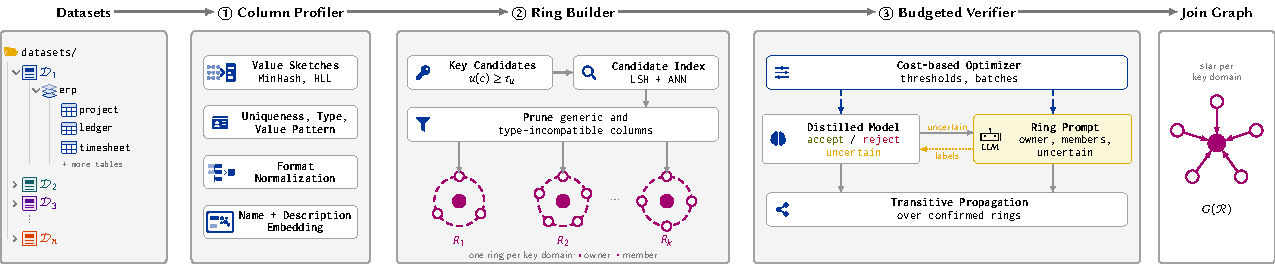
\includegraphics{figures/img/fig_KeyRing_Architecture}}
    \caption{\ourmethod architecture: the \textbf{Column Profiler} summarizes every column in one pass without the LLM; the \textbf{Ring Builder} groups candidate key columns into rings, one per key domain, each with an owner; the \textbf{Budgeted Verifier} accepts or rejects confident candidates with a distilled model, verifies each ring with one batched LLM prompt, and propagates joins by transitivity, so that the join graph keeps a target recall of the all-pairs LLM baseline.}
    \label{fig:system_arch}
\end{figure*}

\introparagraph{Design Principles}
Three principles shape \ourmethod, each serving requirements from Section~\ref{sec:problem}.
First, \ourmethod decides key domains, not table pairs.
The LLM verifies a ring once, and the joins of all its members follow from that answer, so the number of LLM calls grows with the number of key domains (R2), and the output is a star around each owner (R4).
Second, \ourmethod uses each signal for what it is reliable at.
Uniqueness, containment, and embeddings are reliable for proposing candidates, but not for deciding what a column means.
The Ring Builder therefore tunes them for recall, because a join it drops cannot be recovered later, and leaves meaning to the LLM.
Third, \ourmethod pays for the LLM only where its answer changes the outcome, and it reuses every answer it pays for.
A local model, trained only on \ourmethod's own LLM answers, decides confident candidates (R3), and a cost-based optimizer sets its thresholds so that the result meets the recall target (R1).

\subsection{Column Profiler}
\label{sec:arch_profiler}
The Column Profiler makes one pass over the data and computes a profile for each column $c \in \mathcal{C}$.
The profile has four parts, shown on the left of Figure~\ref{fig:system_arch}.
First, \emph{value sketches}: a MinHash sketch of the distinct values for containment estimates~\cite{DBLP:journals/pvldb/ZhuNPM16}, and a HyperLogLog sketch for the number of distinct values.
Second, \emph{statistics}: the uniqueness $u(c)$, the null ratio, the data type, and a value pattern, such as ``three letters, a dash, and five digits''.
Third, \emph{normalized formats}: the profiler strips leading zeros, prefixes, and case differences, and sketches the normalized values as well, so that a join with zero exact overlap can still show containment.
Fourth, an \emph{embedding} of the column name together with its LLM annotation, if the annotation step of the current pipeline (Section~\ref{sec:bg_llm}) has already produced one.
The cost of profiling is linear in the size of the data, and no later step reads raw data again.

\subsection{Ring Builder}
\label{sec:arch_ringbuilder}
The Ring Builder turns profiles into rings in four steps, shown in the middle of Figure~\ref{fig:system_arch}.
First, it selects \emph{key candidates}: columns with uniqueness $u(c) \geq \tau_u$ and few nulls, which can own a key domain.
Second, it generates \emph{candidate references} for every column with two indexes over the key candidates: a containment index on the value sketches~\cite{DBLP:journals/pvldb/ZhuNPM16}, and an approximate nearest-neighbor index on the embeddings.
The first index finds references with overlapping values, and the second finds references whose values differ in format but whose names and descriptions match.
Third, it \emph{prunes} candidates that cannot be keys: columns whose type is incompatible with the owner, and generic columns, such as \texttt{DATA} or small status codes, that match a large fraction of all key candidates.
Fourth, it \emph{forms rings}.
Each key candidate with at least one remaining reference starts a ring, and each referencing column joins the ring of its best-scoring owner.
When two owners reference each other, such as a master table and its staging copy, the Ring Builder merges their rings and elects the owner with the larger domain.
The output is a set of candidate rings, each with an owner, its members, and a score for each member.
Section~\ref{sec:ring_builder} describes these steps in detail.

\subsection{Budgeted Verifier}
\label{sec:arch_verifier}
The Budgeted Verifier turns candidate rings into confirmed rings in four steps, shown on the right of Figure~\ref{fig:system_arch}.
First, the \emph{cost-based optimizer} draws a random sample of candidates and asks the LLM about them.
From these answers, it sets two thresholds on the score of the distilled model, so that the result keeps a target recall $\gamma$ of the oracle with probability at least $1-\delta$, in the style of SUPG and BARGAIN~\cite{SUPG,BARGAIN}.
It also chooses how many candidates to place in one prompt.
Second, the \emph{distilled model} scores every remaining candidate from its profile features.
It accepts candidates above the upper threshold and rejects candidates below the lower threshold.
Third, the \emph{ring prompt} verifies each ring that still has uncertain members.
One prompt contains the owner, the accepted members, and the uncertain candidates of a ring, and the LLM confirms the owner and returns the members that refer to it.
Every LLM answer becomes a label, so the distilled model improves while the verifier runs.
Fourth, \emph{transitive propagation} derives the remaining joins: every confirmed member joins its owner, and two members of the same ring join through it.
The output is the join graph $G(\mathcal{R})$ of Section~\ref{sec:problem}.
Section~\ref{sec:verifier} describes the optimizer and its guarantee.

\begin{example}[Running Example]
In the services firm of Section~\ref{sec:introduction}, the profiler computes the profile of the project master's \texttt{PROJECT\_CODE}, which is unique, and of the $k$ columns that reference it.
Normalization removes the leading zeros of the padded export, so its codes are contained in the master again.
The containment index proposes \texttt{PRJ\_ID} and the padded column as references, and the embedding index proposes \texttt{ENGAGEMENT}, whose values carry a prefix.
The Ring Builder prunes \texttt{DATA}, which matches \todo{X}\% of all key candidates, and merges the staging copy of the master into the same ring.
The distilled model accepts the confident members and rejects the surrogate \texttt{ID} columns, whose values are contained in the codes by accident.
The LLM then verifies the ring with a single prompt that lists the uncertain members, instead of answering $\binom{k+1}{2}$ pairwise prompts.
\end{example}

\section{Column Profiling and Ring Building}
\label{sec:ring_builder}
\todo{Key candidate selection, the two candidate indexes, pruning of generic columns, ring formation and owner election, complexity.}

\section{Budgeted Verification}
\label{sec:verifier}
\todo{Distilled model, threshold selection with recall guarantee, ring prompts and batching, transitive propagation, cost analysis.}

\section{Experiments}
\label{sec:experiments}
\todo{Datasets, baselines (non-LLM, all-pairs LLM, hybrid), cost and quality results.}

\section{Conclusion}
\label{sec:conclusion}
\todo{Conclusion.}


\balance
\bibliographystyle{ACM-Reference-Format}
\bibliography{bib/topic-datalake,bib/topic-modellake,bib/topic-others,bib/topic-ourgroup,bib/topic-llm,bib/topic-scitable,bib/topic-keyring}


\end{document}
